\documentclass[hyperref={pdfpagelabels=false}]{beamer}
\let\Tiny=\tiny
\usepackage{amsmath,amsfonts,amsthm,amssymb}
\usepackage{color}
\usepackage{movie15}
\usepackage{eulervm}
\usepackage{palatino}
%\usepackage{concrete}
%\usepackage{charter}
%\usepackage{courier}
% \usetheme{Warsaw}
% \usefonttheme{serif}
\usetheme{Singapore}

\title{Kalman Filter for Unicycle-like Robots}
\author{Thomas Denewiler}
%\institute{UCSD/SPAWAR}
\institute{SPAWAR}
%\date{June 22, 2010}

\begin{document}

% Define new variables.
\def\argmin{\mathop{\arg\,\min}\limits}
\def\argmax{\mathop{\arg\,\max}\limits}

\begin{frame}
\titlepage
\end{frame}

\begin{frame}{Outline}
\begin{itemize}
\item Overview.
\item A first look at the algorithm.
\item States.
\item Assumptions to simplify the system model.
\item Predicting states with the system model.
\item Handling sensor data with the measurement model.
\item Revisit algorithm.
\item Noise models, covariance and gain.
\item Example to estimate yaw state with noisy sensors.
\item Identifying noise models.
\item Alternate estimation methods.
\item Algorithm one last time.
\item References.
\end{itemize}
\end{frame}

\begin{frame}{Overview}
\begin{itemize}
\item Kalman filter answers question "Where am I?"
\item Unicycle-like robots are differential drive, or skid-steer, robots like the EOD robots.
\item There are several states of interest including position, orientation and linear and angular velocities.
\item Multiple sensors are measuring the states. Some states are not measured, only estimated.
\item There are four models, one that describes how the system moves through time, one for the measurements, one for system noise and one for sensor noise.
\item The Kalman filter merges the model and sensor data to estimate the state variables in the presence of missing or conflicting measurements, noise and incomplete, simplified models.
\end{itemize}
\end{frame}

\begin{frame}{Caveats}
\begin{itemize}
\item This is not a derivation.
\item This is not mathematically rigorous.
\item Many good books and tutorials exist for derivation, several listed in References.
\item Intent is to show where equations in code come from and to give an idea of what will result when tweaking the parameters.
\item ACS and MPRS Kalman filter implementations use the models described here.
\end{itemize}
\end{frame}

\begin{frame}{Basic Ideas}
The Kalman filter algorithm consists of two main steps:
\begin{itemize}
\item Prediction update step based on system model.
\item Measurement update step based on sensor data.
\end{itemize}
\begin{figure}[ht!]
	\centering
	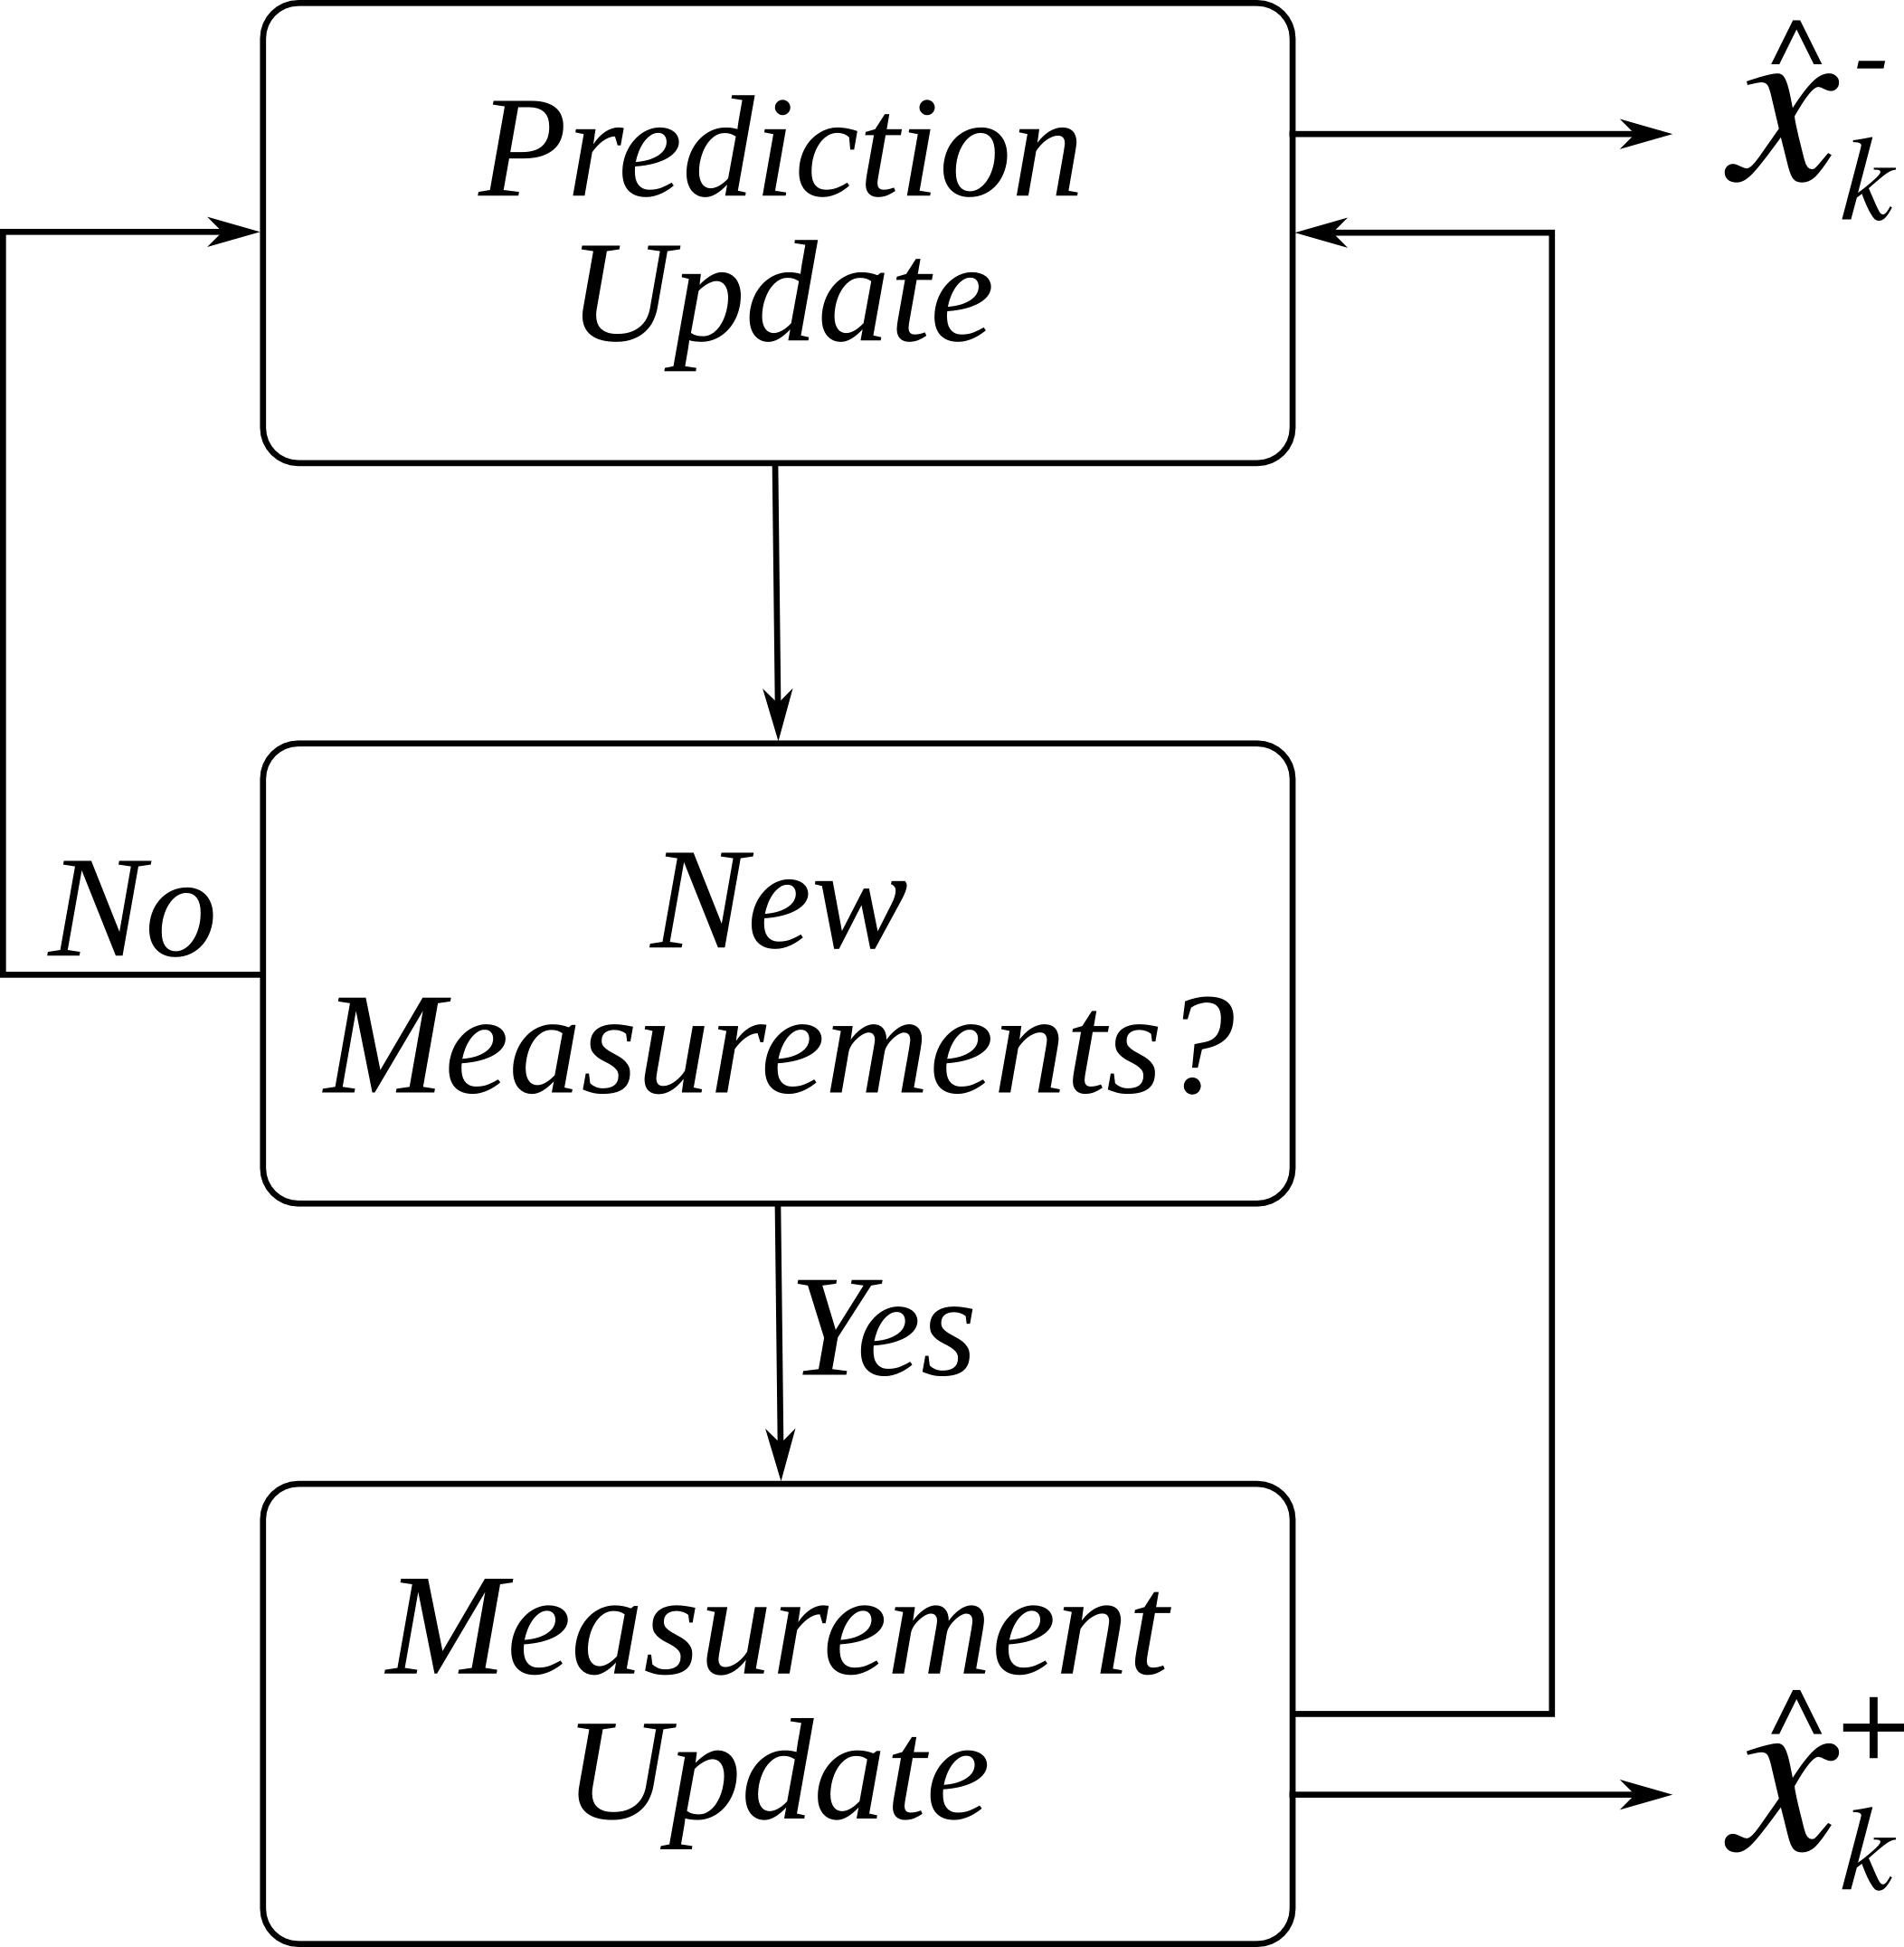
\includegraphics[width=.3\textwidth]{images/kf}
\end{figure}
\end{frame}

\begin{frame}{Algorithm - Focus on $\hat{x}$}
\begin{itemize}
\item A generic system is represented by the model
\begin{align*}
x_{k+1} &= \Phi_kx_k + w_k \\
y_k &= H_kx_k + v_k
\end{align*}
\item Prediction update equations.
\begin{align*}
\hat{x}_{k+1}^- &= \Phi_k\hat{x}_k^+ \\
P_{k+1}^- &= \Phi_kP_k^+\Phi_k^T + Q_k
\end{align*}
\item Measurement update equations.
\begin{align*}
K_k &= P_k^-H_k^T\left[H_kP_k^-H_k^T + R_k\right]^{-1} \\
\hat{x}_k^+ &= \hat{x}_k^- + K_k\left[y_k - H_k\hat{x}_k^-\right] \\
P_k^+ &= \left[I - K_kH_k\right]P_k^-
\end{align*}
\end{itemize}
\end{frame}

\begin{frame}{Extended Kalman Filter}
\begin{itemize}
\item The standard Kalman filter is based on the model
\begin{align*}
x_{k+1} &= \Phi_kx_k + w_k \\
y_k &= H_kx_k + v_k
\end{align*}
where the calculation of the next state is based on the current state.
\item Kalman filter requires linear systems.
\item Linear systems \textit{do not exist}.
\item Nonlinear systems can be approximated by linear systems with varying degrees of success. The key is how fast systems change at each time step.
\item Systems change based on their dynamics.
\item The extended Kalman filter linearizes nonlinear models and then uses the standard Kalman filter equations.
\end{itemize}
\end{frame}

\begin{frame}{Linearizing Models}
\begin{itemize}
\item Effects of linearizing a nonlinear model.
\item The derivative of the nonlinear system is evaluated at the current state to get a linear approximation.
\item If the dynamics are too fast then the linear approximation will give inaccurate results.
\end{itemize}
\begin{figure}[ht!]
    \centering
    \includegraphics[width=.9\textwidth]{images/KFLinearization2}
\end{figure}
\end{frame}

\begin{frame}{Robot States}
\begin{itemize}
\item The states are $x$, $y$, $z$ positions, $\theta$, $\phi$, $\psi$ Euler angles (pitch, roll, yaw) and $V$, $\omega$ velocities (linear, angular).
\item Body frame coordinate system.
\item A coordinate frame transformation is needed to convert to world coordinate system.
\end{itemize}
\begin{figure}[ht!]
    \centering
    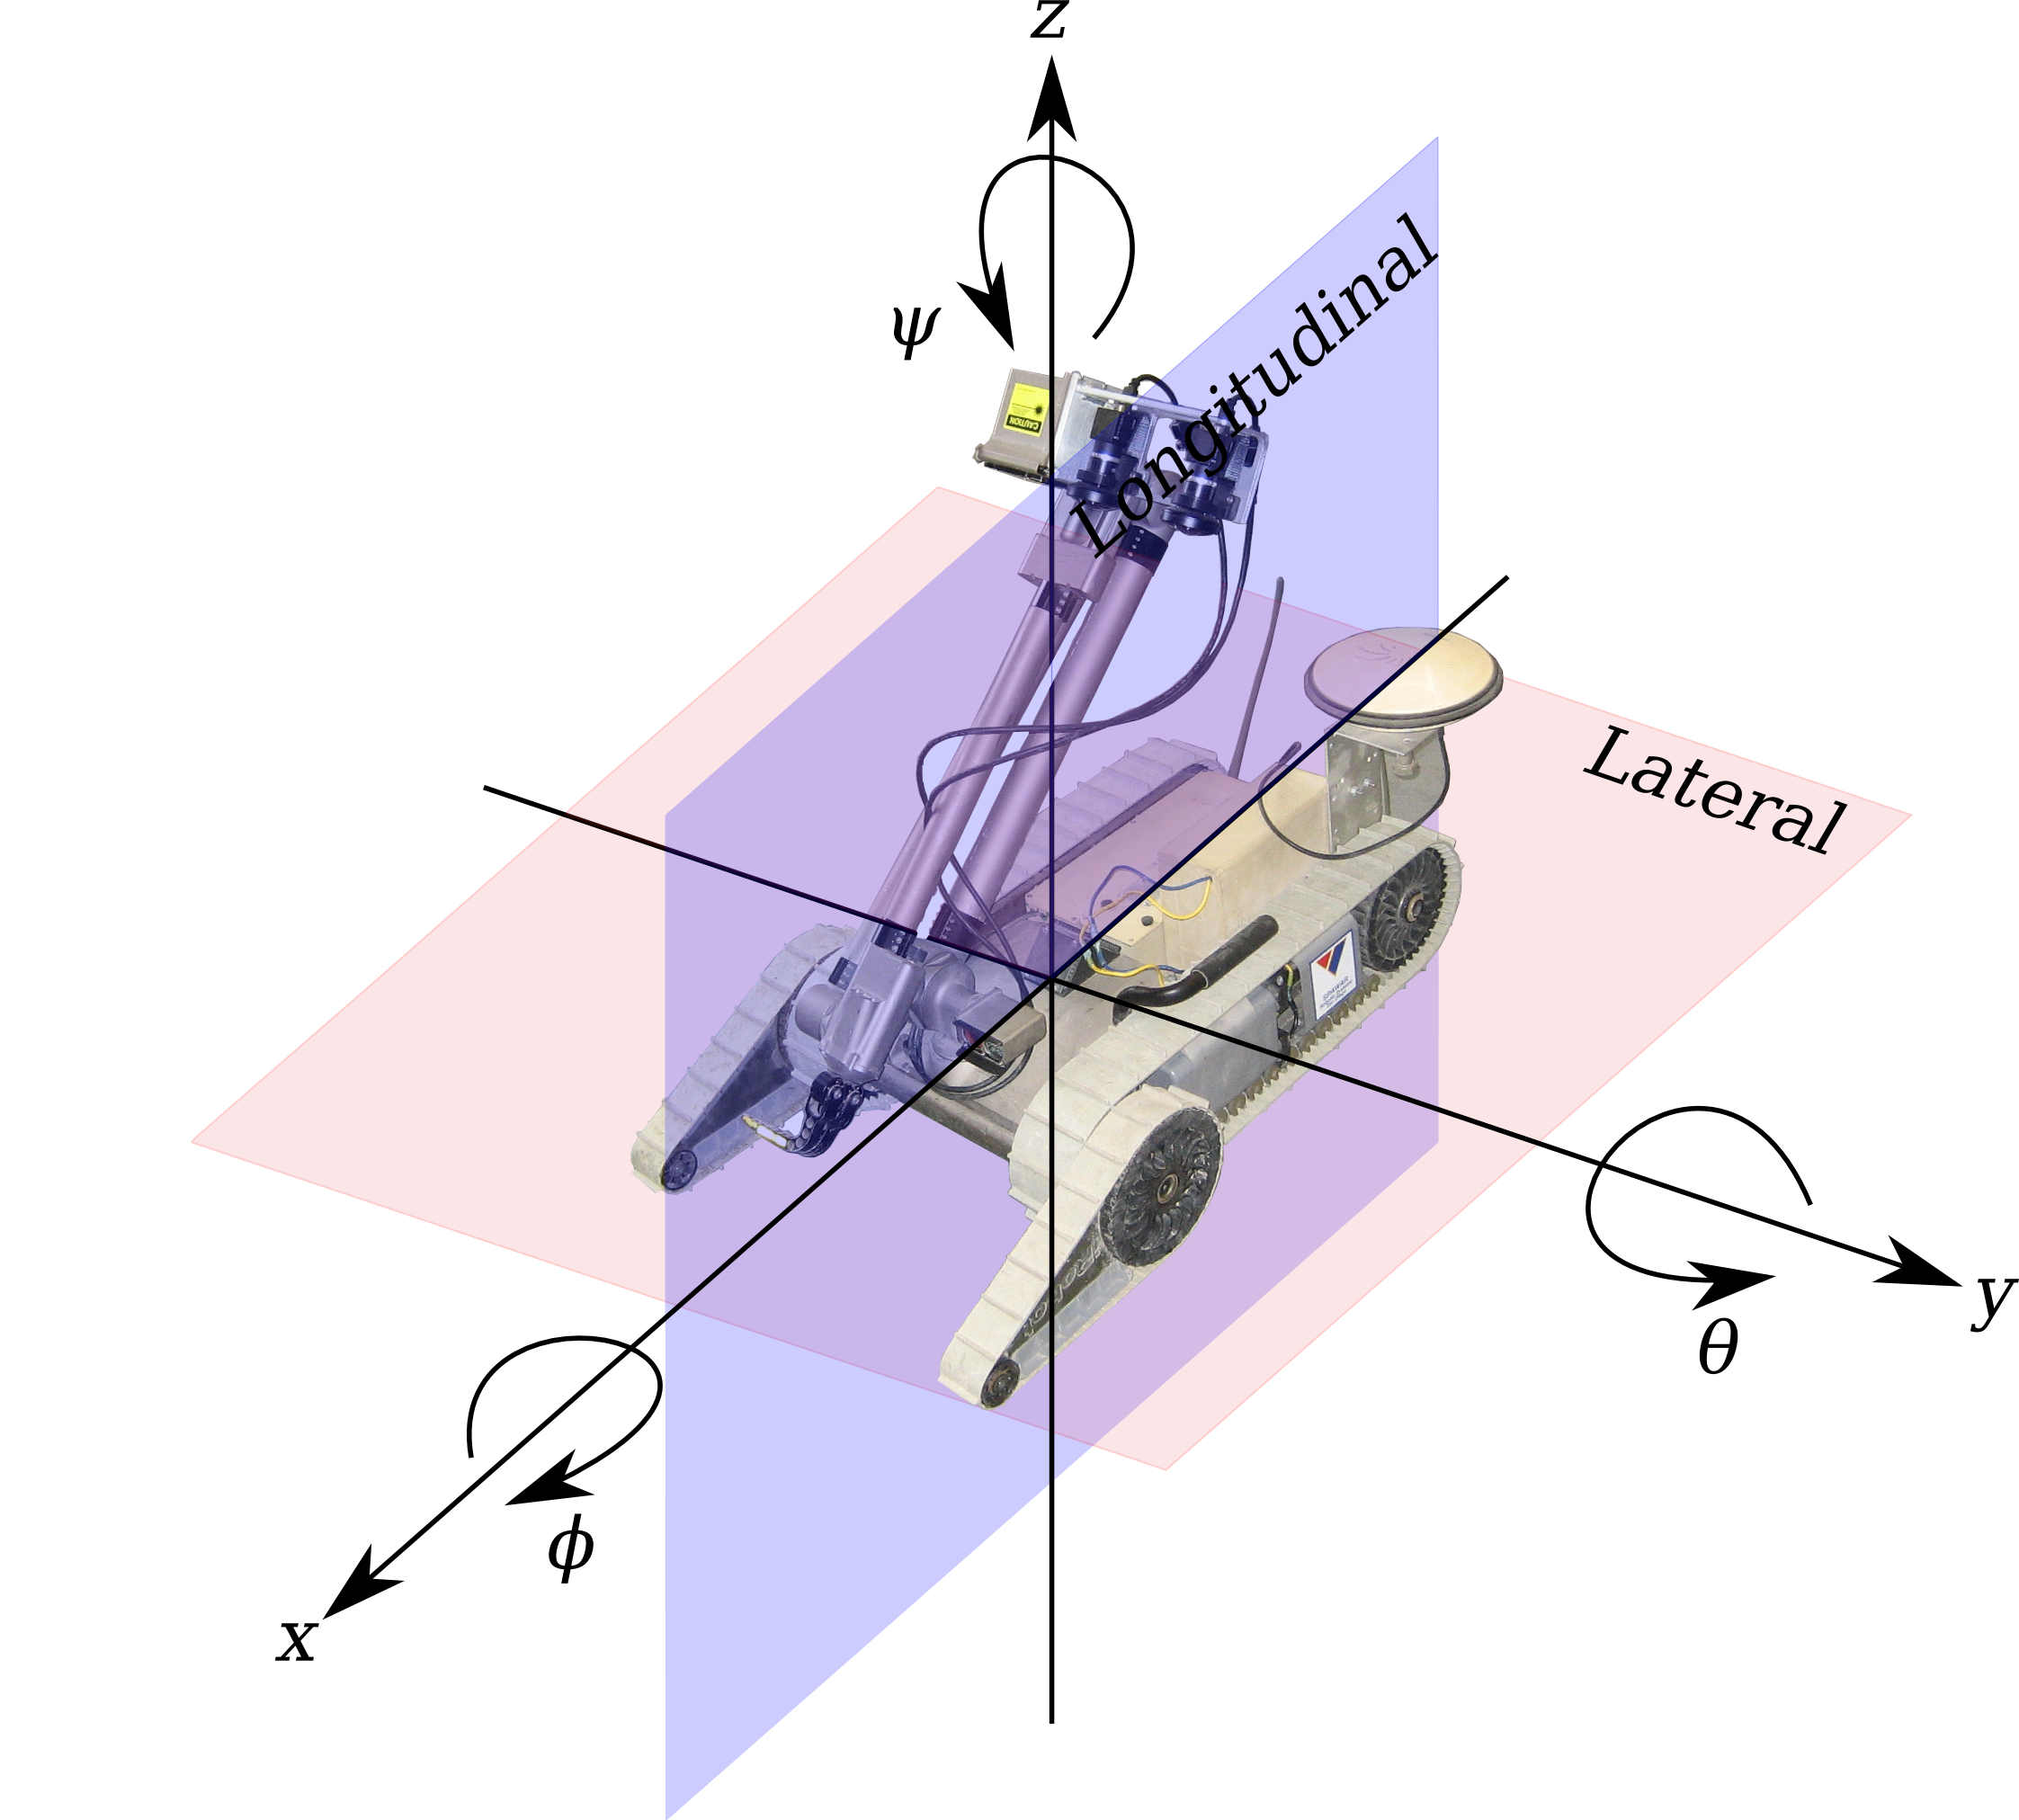
\includegraphics[width=.5\textwidth]{images/packbotaxes}
\end{figure}
\end{frame}

\begin{frame}{Low Dynamics Assumption}
\begin{itemize}
\item For the duration of a single time step the linear and angular velocities do not change by a measurable amount.
\item Assume that the velocities are constant.
\item Reduces the number of states by six due to accelerations about each axis of motion.
\item Valid when accelerations of the robot are at or near the level of the noise of the sensor measuring accelerations.
\end{itemize}
\end{frame}

\begin{frame}{Principal Motion Assumption}
\begin{itemize}
\item For the duration of a single time step the position estimates are only influenced by the linear velocity (and not the angular velocity) of the robot.
\item The Euler angles (orientation) are only influenced by the angular velocity of the robot.
\item Allows several terms in the system model $\Phi$ to be set to zero.
\end{itemize}
\end{frame}

\begin{frame}{System Model}
\begin{itemize}
\item A nonlinear model based on the robot kinematics.
\item In body frame coordinate system.
\item $\dot{x} = f(x)$
\end{itemize}
\begin{align*}
\frac{d}{dt}\left[\begin{array}{c}
x \\ y \\ z \\ V \\ \theta \\ \phi \\ \psi \\ \omega
\end{array}\right] =
\left[\begin{array}{c}
V\cos\psi\cos\theta \\
V\sin\psi\cos\theta \\
-V\sin\theta \\
0 \\
-\omega\sin\phi \\
\omega\tan\theta\cos\phi \\
\omega\cos\phi/\cos\theta \\
0
\end{array}\right]
\end{align*}
\end{frame}

\begin{frame}{Computing A Linearized System Model}
\begin{itemize}
\item For the extended Kalman filter the system model is linearized.
\item The derivative of each element of the nonlinear model is taken with respect to the state that it is associated with.
\item Attempting to get a valid approximation to nonlinear model.
\end{itemize}
{\tiny
\begin{align*}
\dot{x} =
\underbrace{\left[\begin{array}{c c c c c c c c}
\frac{\partial \dot{x}}{\partial x} & \frac{\partial \dot{x}}{\partial y} & \frac{\partial \dot{x}}{\partial z} & \frac{\partial \dot{x}}{\partial V} & \frac{\partial \dot{x}}{\partial \theta} & \frac{\partial \dot{x}}{\partial \phi} & \frac{\partial \dot{x}}{\partial \psi} & \frac{\partial \dot{x}}{\partial \omega} \\
\frac{\partial \dot{y}}{\partial x} & \frac{\partial \dot{y}}{\partial y} & \frac{\partial \dot{y}}{\partial z} & \frac{\partial \dot{y}}{\partial V} & \frac{\partial \dot{y}}{\partial \theta} & \frac{\partial \dot{y}}{\partial \phi} & \frac{\partial \dot{y}}{\partial \psi} & \frac{\partial \dot{y}}{\partial \omega} \\
\frac{\partial \dot{z}}{\partial x} & \frac{\partial \dot{z}}{\partial y} & \frac{\partial \dot{z}}{\partial z} & \frac{\partial \dot{z}}{\partial V} & \frac{\partial \dot{z}}{\partial \theta} & \frac{\partial \dot{z}}{\partial \phi} & \frac{\partial \dot{z}}{\partial \psi} & \frac{\partial \dot{z}}{\partial \omega} \\
\frac{\partial \dot{V}}{\partial x} & \frac{\partial \dot{V}}{\partial y} & \frac{\partial \dot{V}}{\partial z} & \frac{\partial \dot{V}}{\partial V} & \frac{\partial \dot{V}}{\partial \theta} & \frac{\partial \dot{V}}{\partial \phi} & \frac{\partial \dot{V}}{\partial \psi} & \frac{\partial \dot{V}}{\partial \omega} \\
\frac{\partial \dot{\theta}}{\partial x} & \frac{\partial \dot{\theta}}{\partial y} & \frac{\partial \dot{\theta}}{\partial z} & \frac{\partial \dot{\theta}}{\partial V} & \frac{\partial \dot{\theta}}{\partial \theta} & \frac{\partial \dot{\theta}}{\partial \phi} & \frac{\partial \dot{\theta}}{\partial \psi} & \frac{\partial \dot{\theta}}{\partial \omega} \\
\frac{\partial \dot{\phi}}{\partial x} & \frac{\partial \dot{\phi}}{\partial y} & \frac{\partial \dot{\phi}}{\partial z} & \frac{\partial \dot{\phi}}{\partial V} & \frac{\partial \dot{\phi}}{\partial \theta} & \frac{\partial \dot{\phi}}{\partial \phi} & \frac{\partial \dot{\phi}}{\partial \psi} & \frac{\partial \dot{\phi}}{\partial \omega} \\
\frac{\partial \dot{\psi}}{\partial x} & \frac{\partial \dot{\psi}}{\partial y} & \frac{\partial \dot{\psi}}{\partial z} & \frac{\partial \dot{\psi}}{\partial V} & \frac{\partial \dot{\psi}}{\partial \theta} & \frac{\partial \dot{\psi}}{\partial \phi} & \frac{\partial \dot{\psi}}{\partial \psi} & \frac{\partial \dot{\psi}}{\partial \omega} \\
\frac{\partial \dot{\omega}}{\partial x} & \frac{\partial \dot{\omega}}{\partial y} & \frac{\partial \dot{\omega}}{\partial z} & \frac{\partial \dot{\omega}}{\partial V} & \frac{\partial \dot{\omega}}{\partial \theta} & \frac{\partial \dot{\omega}}{\partial \phi} & \frac{\partial \dot{\omega}}{\partial \psi} & \frac{\partial \dot{\omega}}{\partial \omega}
\end{array}\right]}_{F}
\left[\begin{array}{c}
x \\ y \\ z \\ V \\ \theta \\ \phi \\ \psi \\ \omega
\end{array}\right]
\end{align*}
}
\end{frame}

\begin{frame}{Linearized System Model Results}
\begin{itemize}
\item The derivatives are known analytically so they can be calculated in advance and not at each time step.
\item $\dot{x} = Fx$
\end{itemize}
{\tiny
\begin{align*}
\frac{d}{dt}\left[\begin{array}{c}
\Delta x \\ \Delta y \\ \Delta z \\ \Delta V \\ \Delta \theta \\ \Delta \phi \\ \Delta \psi \\ \Delta \omega
\end{array}\right] =
\underbrace{\left[\begin{array}{c c c c c c c c}
0 & 0 & 0 & c\psi c\theta & -V c\psi s\theta               & 0                     & -V s\psi c\theta & 0 \\
0 & 0 & 0 & s\psi c\theta & -V s\psi s\theta               & 0                     & V c\psi c\theta  & 0 \\
0 & 0 & 0 & -s\theta      & -V c\theta                     & 0                     & 0                & 0 \\
0 & 0 & 0 & 0             & 0                              & 0                     & 0                & 0 \\
0 & 0 & 0 & 0             & 0                              & -\omega c\phi         & 0                & -s\phi \\
0 & 0 & 0 & 0             & \omega c\phi/c^2\theta         & \omega t\theta s\phi  & 0                & t\theta c\phi \\
0 & 0 & 0 & 0             & \omega s\theta c\phi/c^2\theta & -\omega s\phi/c\theta & 0                & c\phi/c\theta \\
0 & 0 & 0 & 0             & 0                              & 0                     & 0                & 0
\end{array}\right]}_{F}
\left[\begin{array}{c}
\Delta x \\ \Delta y \\ \Delta z \\ \Delta V \\ \Delta \theta \\ \Delta \phi \\ \Delta \psi \\ \Delta \omega
\end{array}\right]
\end{align*}
}
\end{frame}

\begin{frame}{Transform From Continuous to Discrete Time}
\begin{itemize}
\item Continuous time:
\begin{align*}
\dot{x} = Fx
\end{align*}
\item Discrete time:
\begin{align*}
x_{k+1} = \Phi_kx_k
\end{align*}
\item Obeys exponential matrix transformation with a Taylor series approximation:
\begin{align*}
\Phi_k = e^{F\Delta_T} = I + F\Delta_T + \frac{(F\Delta_T)^2}{2!} + \ldots + \frac{(F\Delta_T)^n}{n!}
\end{align*}
\item Under the principal motion assumption $F$ is constant and the higher order terms vanish to leave exactly 
\begin{align*}
\Phi_k = I + F\Delta_T
\end{align*}
\end{itemize}
\end{frame}

\begin{frame}{Linearized System Model with Assumptions}
\begin{itemize}
\item The system model is simplified by invoking the low dynamics assumption and the principal motion assumption.
\item Moving from continuous time to discrete time is done by $\Phi_k = I + F\Delta_T$.
\item Positions depend on previous state and linear velocity, orientation on previous state and angular velocity.
\begin{align*}
x_{k+1} = 
\underbrace{\left[\begin{array}{c c c c c c c c}
1 & 0 & 0 & c\psi c\theta \Delta_T & 0 & 0 & 0 & 0 \\
0 & 1 & 0 & s\psi c\theta \Delta_T & 0 & 0 & 0 & 0\\
0 & 0 & 1 & -s\theta \Delta_T & 0 & 0 & 0 & 0\\
0 & 0 & 0 & 1 & 0 & 0 & 0 & 0 \\
0 & 0 & 0 & 0 & 1 & 0 & 0 & -s\phi \Delta_T \\
0 & 0 & 0 & 0 & 0 & 1 & 0 & t\theta c\phi \Delta_T \\
0 & 0 & 0 & 0 & 0 & 0 & 1 & c\phi \Delta_T/c\theta \\
0 & 0 & 0 & 0 & 0 & 0 & 0 & 1
\end{array}\right]}_{\Phi_k}
\left[\begin{array}{c}
x \\ y \\ z \\ V \\ \theta \\ \phi \\ \psi \\ \omega
\end{array}\right]_k
\end{align*}
\end{itemize}
\end{frame}

\begin{frame}{Review of Assumptions}
\begin{itemize}
\item Nonlinear model has no wheel slip, no lateral movement -- non-holonomic vehicle. Those effects go into noise terms.
\item A linear model is good enough as the nonlinear dynamics are indistinguishable from sensor and process noise.
\item Low dynamics assumption.
\item Principal motion assumption.
\end{itemize}
\end{frame}

\begin{frame}{Benefits of Assumptions}
% \transdissolve
\begin{itemize}
\item Original nonlinear model.
\end{itemize}
\begin{align*}
\frac{d}{dt}\left[\begin{array}{c}
x \\ y \\ z \\ V \\ \theta \\ \phi \\ \psi \\ \omega
\end{array}\right] =
\left[\begin{array}{c}
V\sin\psi\cos\theta \\
-V\cos\psi\cos\theta \\
V\cos\theta \\
0 \\
\omega\cos\phi \\
-\omega\tan\theta\cos\phi \\
\omega\sin\phi/\cos\theta \\
0
\end{array}\right]
\end{align*}
\end{frame}

\begin{frame}{Benefits of Assumptions}
% \transdissolve
\begin{itemize}
\item Linearized model.
\end{itemize}
{\tiny
\begin{align*}
\frac{d}{dt}\left[\begin{array}{c}
\Delta x \\ \Delta y \\ \Delta z \\ \Delta V \\ \Delta \theta \\ \Delta \phi \\ \Delta \psi \\ \Delta \omega
\end{array}\right] =
\left[\begin{array}{c c c c c c c c}
0 & 0 & 0 & c\psi c\theta & -V c\psi s\theta               & 0                     & -V s\psi c\theta & 0 \\
0 & 0 & 0 & s\psi c\theta & -V s\psi s\theta               & 0                     & V c\psi c\theta  & 0 \\
0 & 0 & 0 & -s\theta      & -V c\theta                     & 0                     & 0                & 0 \\
0 & 0 & 0 & 0             & 0                              & 0                     & 0                & 0 \\
0 & 0 & 0 & 0             & 0                              & -\omega c\phi         & 0                & -s\phi \\
0 & 0 & 0 & 0             & \omega c\phi/c^2\theta         & \omega t\theta s\phi  & 0                & t\theta c\phi \\
0 & 0 & 0 & 0             & \omega s\theta c\phi/c^2\theta & -\omega s\phi/c\theta & 0                & c\phi/c\theta \\
0 & 0 & 0 & 0             & 0                              & 0                     & 0                & 0
\end{array}\right]
\left[\begin{array}{c}
\Delta x \\ \Delta y \\ \Delta z \\ \Delta V \\ \Delta \theta \\ \Delta \phi \\ \Delta \psi \\ \Delta \omega
\end{array}\right]
\end{align*}
}
\end{frame}

\begin{frame}{Benefits of Assumptions}
% \transdissolve
\begin{itemize}
\item Principal motion assumption. Greatly reduced calculations!
\end{itemize}
{\tiny
\begin{align*}
x_{k+1} = \left[\begin{array}{c c c c c c c c}
1 & 0 & 0 & c\psi c\theta \Delta_T & 0 & 0 & 0 & 0 \\
0 & 1 & 0 & s\psi c\theta \Delta_T & 0 & 0 & 0 & 0\\
0 & 0 & 1 & -s\theta \Delta_T & 0 & 0 & 0 & 0\\
0 & 0 & 0 & 1 & 0 & 0 & 0 & 0 \\
0 & 0 & 0 & 0 & 1 & 0 & 0 & -s\phi \Delta_T \\
0 & 0 & 0 & 0 & 0 & 1 & 0 & t\theta c\phi \Delta_T \\
0 & 0 & 0 & 0 & 0 & 0 & 1 & c\phi \Delta_T/c\theta \\
0 & 0 & 0 & 0 & 0 & 0 & 0 & 1
\end{array}\right]
\left[\begin{array}{c}
x \\ y \\ z \\ V \\ \theta \\ \phi \\ \psi \\ \omega
\end{array}\right]
\end{align*}
}
\end{frame}

\begin{frame}{Measurement Model}
\begin{itemize}
\item Generic system model:
\begin{align*}
x_{k+1} &= F_kx_k + w_k \\
y_k &= H_kx_k + v_k
\end{align*}
\item $H$ transforms the state coordinates into sensor data coordinates.
\item With 8 states, measuring all once and yaw twice:
\begin{align*}
H = \left[\begin{array}{c c c c c c c c}
1 & 0 & 0 & 0 & 0 & 0 & 0 & 0 \\
0 & 1 & 0 & 0 & 0 & 0 & 0 & 0 \\
0 & 0 & 1 & 0 & 0 & 0 & 0 & 0 \\
0 & 0 & 0 & 1 & 0 & 0 & 0 & 0 \\
0 & 0 & 0 & 0 & 1 & 0 & 0 & 0 \\
0 & 0 & 0 & 0 & 0 & 1 & 0 & 0 \\
0 & 0 & 0 & 0 & 0 & 0 & 1 & 0 \\
0 & 0 & 0 & 0 & 0 & 0 & \frac{180^\circ}{\pi} & 0 \\
0 & 0 & 0 & 0 & 0 & 0 & 0 & 1
\end{array}\right]
\end{align*}
\end{itemize}
\end{frame}

\begin{frame}{Algorithm Revisited - Focus Still on $\hat{x}$}
\begin{itemize}
\item A generic system is represented by the model
\begin{align*}
x_{k+1} &= \Phi_kx_k + w_k \\
y_k &= H_kx_k + v_k
\end{align*}
\item Prediction update equations
\begin{align*}
\hat{x}_{k+1}^- &= \Phi_k\hat{x}_k^+ \\
P_{k+1}^- &= \Phi_kP_k^+\Phi_k^T + Q_k
\end{align*}
\item Measurement update equations
\begin{align*}
K_k &= P_k^-H_k^T\left[H_kP_k^-H_k^T + R_k\right]^{-1} \\
\hat{x}_k^+ &= \hat{x}_k^- + K_k\left[y_k - H_k\hat{x}_k^-\right] \\
P_k^+ &= \left[I - K_kH_k\right]P_k^-
\end{align*}
\end{itemize}
\end{frame}

\begin{frame}{Noise Models - Determining Covariances}
\begin{itemize}
\item Keep track of covariance for system, measurements and estimate.
\item System covariance $Q$ is the uncertainty in the state model during time interval between measurements when estimate is found using system model.
\item Measurement covariance $R$ is the uncertainty of the sensors.
\item Can be set \textit{a priori} from manufacturers data sheets or through testing using system identification techniques.
\item Can be calculated online in real time.
\item Covariance of the state estimate is in $P$ and is updated in the Kalman filter equations.
\end{itemize}
\end{frame}

\begin{frame}{Kalman Gain}
\begin{itemize}
\item Kalman gain is:
\begin{align*}
K_k &= P_k^-H_k^T\left[H_kP_k^-H_k^T + R_k\right]^{-1}
\end{align*}
\item Low gain weights estimate from system model more than measurement.
\item High gain weights measurement more than estimate from system model.
\item Gain is based on all four models -- system model $\Phi$, system noise model $Q$, measurement model $H$ and measurement noise model $R$.
\end{itemize}
\end{frame}

\begin{frame}{Innovations - Using New Data}
\begin{itemize}
\item New sensor data gives new information about the state of the robot and its environment.
\item Measurements are used to update system model estimate.
\item The key concept is that the difference between expected measurement values and actual measurements is used to generate new state estimate.
\item New measurements: $y_k$. Expected measurements: $H_k\hat{x}_k$.
\item Difference, or "innovations", multiplied by Kalman gain to adjust previous state estimate from system model:
\begin{align*}
\hat{x}_k^+ &= \hat{x}_k^- + K_k\left[y_k - H_k\hat{x}_k^-\right]
\end{align*}
\end{itemize}
\end{frame}

\begin{frame}{Example - Estimating Yaw}
\begin{itemize}
\item Same system model developed above. Assume sensors measuring ground truth.
\item Two yaw sensors with adjustable noise and drift.
\item Kalman filter estimate is much closer to better sensor.
\item Yaw sensor 1 noise is $v_{\psi_1} = 1^\circ$, yaw sensor 2 noise is $v_{\psi_1} = 5^\circ$.
\item Typical RMS error results for estimates with no drift.
\begin{itemize}
\item Position = $0.0$ meters.
\item Yaw = $0.023$ radians = $1.359^\circ$.
\end{itemize}
\end{itemize}
\end{frame}

\begin{frame}{Example - Estimating Yaw - Measurement Model}
\begin{itemize}
\item Using 9 sensors total, 2 for yaw.
\item Assume yaw sensor 1 measures in radians, yaw sensor 2 measures in degrees, yaw state in radians.
\begin{itemize}
\item $H$ transforms yaw state from radians to degrees so that error $y-H\hat{x}$ can be calculated.
\end{itemize}
\item One row per sensor, one column per state.
\end{itemize}
\begin{align*}
y = \underbrace{\left[\begin{array}{c c c c c c c c}
1 & 0 & 0 & 0 & 0 & 0 & 0 & 0 \\
0 & 1 & 0 & 0 & 0 & 0 & 0 & 0 \\
0 & 0 & 1 & 0 & 0 & 0 & 0 & 0 \\
0 & 0 & 0 & 1 & 0 & 0 & 0 & 0 \\
0 & 0 & 0 & 0 & 1 & 0 & 0 & 0 \\
0 & 0 & 0 & 0 & 0 & 1 & 0 & 0 \\
0 & 0 & 0 & 0 & 0 & 0 & 1 & 0 \\
0 & 0 & 0 & 0 & 0 & 0 & \frac{180^\circ}{\pi} & 0 \\
0 & 0 & 0 & 0 & 0 & 0 & 0 & 1
\end{array}\right]}_{H}
\left[\begin{array}{c}
x \\ y \\ z \\ V \\ \theta \\ \phi \\ \psi \\ \omega
\end{array}\right]
\end{align*}
\end{frame}

\begin{frame}{Example - Estimating Yaw - Single Measurement}
\begin{itemize}
\item The measurement model $H$ changes based on number of measurements.
\item Zeroes out states without new data.
\item For zeroed states the measurement update step leaves $\hat{x}_k^+ = \hat{x}_k^-$ based on $\hat{x}_k^+ = \hat{x}_k^- + K_k\left[y_k - H_k\hat{x}_k^-\right]$.
\end{itemize}
\begin{align*}
\hat{y}_k = \underbrace{\left[\begin{array}{c c c c c c c c}
0 & 0 & 0 & 0 & 0 & 0 & \frac{180^\circ}{\pi} & 0 \\
\end{array}\right]}_{H}
\left[\begin{array}{c}
x \\ y \\ z \\ V \\ \theta \\ \phi \\ \psi \\ \omega
\end{array}\right]
\end{align*}
\end{frame}

\begin{frame}{Example - Estimating Yaw - System Covariance}
\begin{itemize}
\item Where do we expect the system model to be inaccurate?
\item For this example assume the model is correct.
\end{itemize}
\begin{align*}
Q = \left[\begin{array}{c c c c c c c c}
1 & 0 & 0 & 0 & 0 & 0 & 0 & 0 \\
0 & 1 & 0 & 0 & 0 & 0 & 0 & 0 \\
0 & 0 & 1 & 0 & 0 & 0 & 0 & 0 \\
0 & 0 & 0 & 1 & 0 & 0 & 0 & 0 \\
0 & 0 & 0 & 0 & 1 & 0 & 0 & 0 \\
0 & 0 & 0 & 0 & 0 & 1 & 0 & 0 \\
0 & 0 & 0 & 0 & 0 & 0 & 1 & 0 \\
0 & 0 & 0 & 0 & 0 & 0 & 0 & 1
\end{array}\right]
\end{align*}
\end{frame}

\begin{frame}{Example - Estimating Yaw - Measurement Covariance}
\begin{itemize}
\item Where do we expect the measurements to be inaccurate?
\item For this example we know that the yaw sensors are not correct and we know how much noise to expect for each sensor, $v_{\psi_1}$ and $v_{\psi_2}$.
\end{itemize}
\begin{align*}
R = \left[\begin{array}{c c c c c c c c c}
0 & 0 & 0 & 0 & 0 & 0 & 0 & 0 & 0 \\
0 & 0 & 0 & 0 & 0 & 0 & 0 & 0 & 0 \\
0 & 0 & 0 & 0 & 0 & 0 & 0 & 0 & 0 \\
0 & 0 & 0 & 0 & 0 & 0 & 0 & 0 & 0 \\
0 & 0 & 0 & 0 & 0 & 0 & 0 & 0 & 0 \\
0 & 0 & 0 & 0 & 0 & 0 & 0 & 0 & 0 \\
0 & 0 & 0 & 0 & 0 & 0 & v_{\psi_1} & 0 & 0 \\
0 & 0 & 0 & 0 & 0 & 0 & 0 & v_{\psi_2} & 0 \\
0 & 0 & 0 & 0 & 0 & 0 & 0 & 0 & 0
\end{array}\right]
\end{align*}
\end{frame}

\begin{frame}{Example - Estimating Yaw - Results}
\begin{figure}[ht!]
    \centering
    \begin{tabular}{c c}
    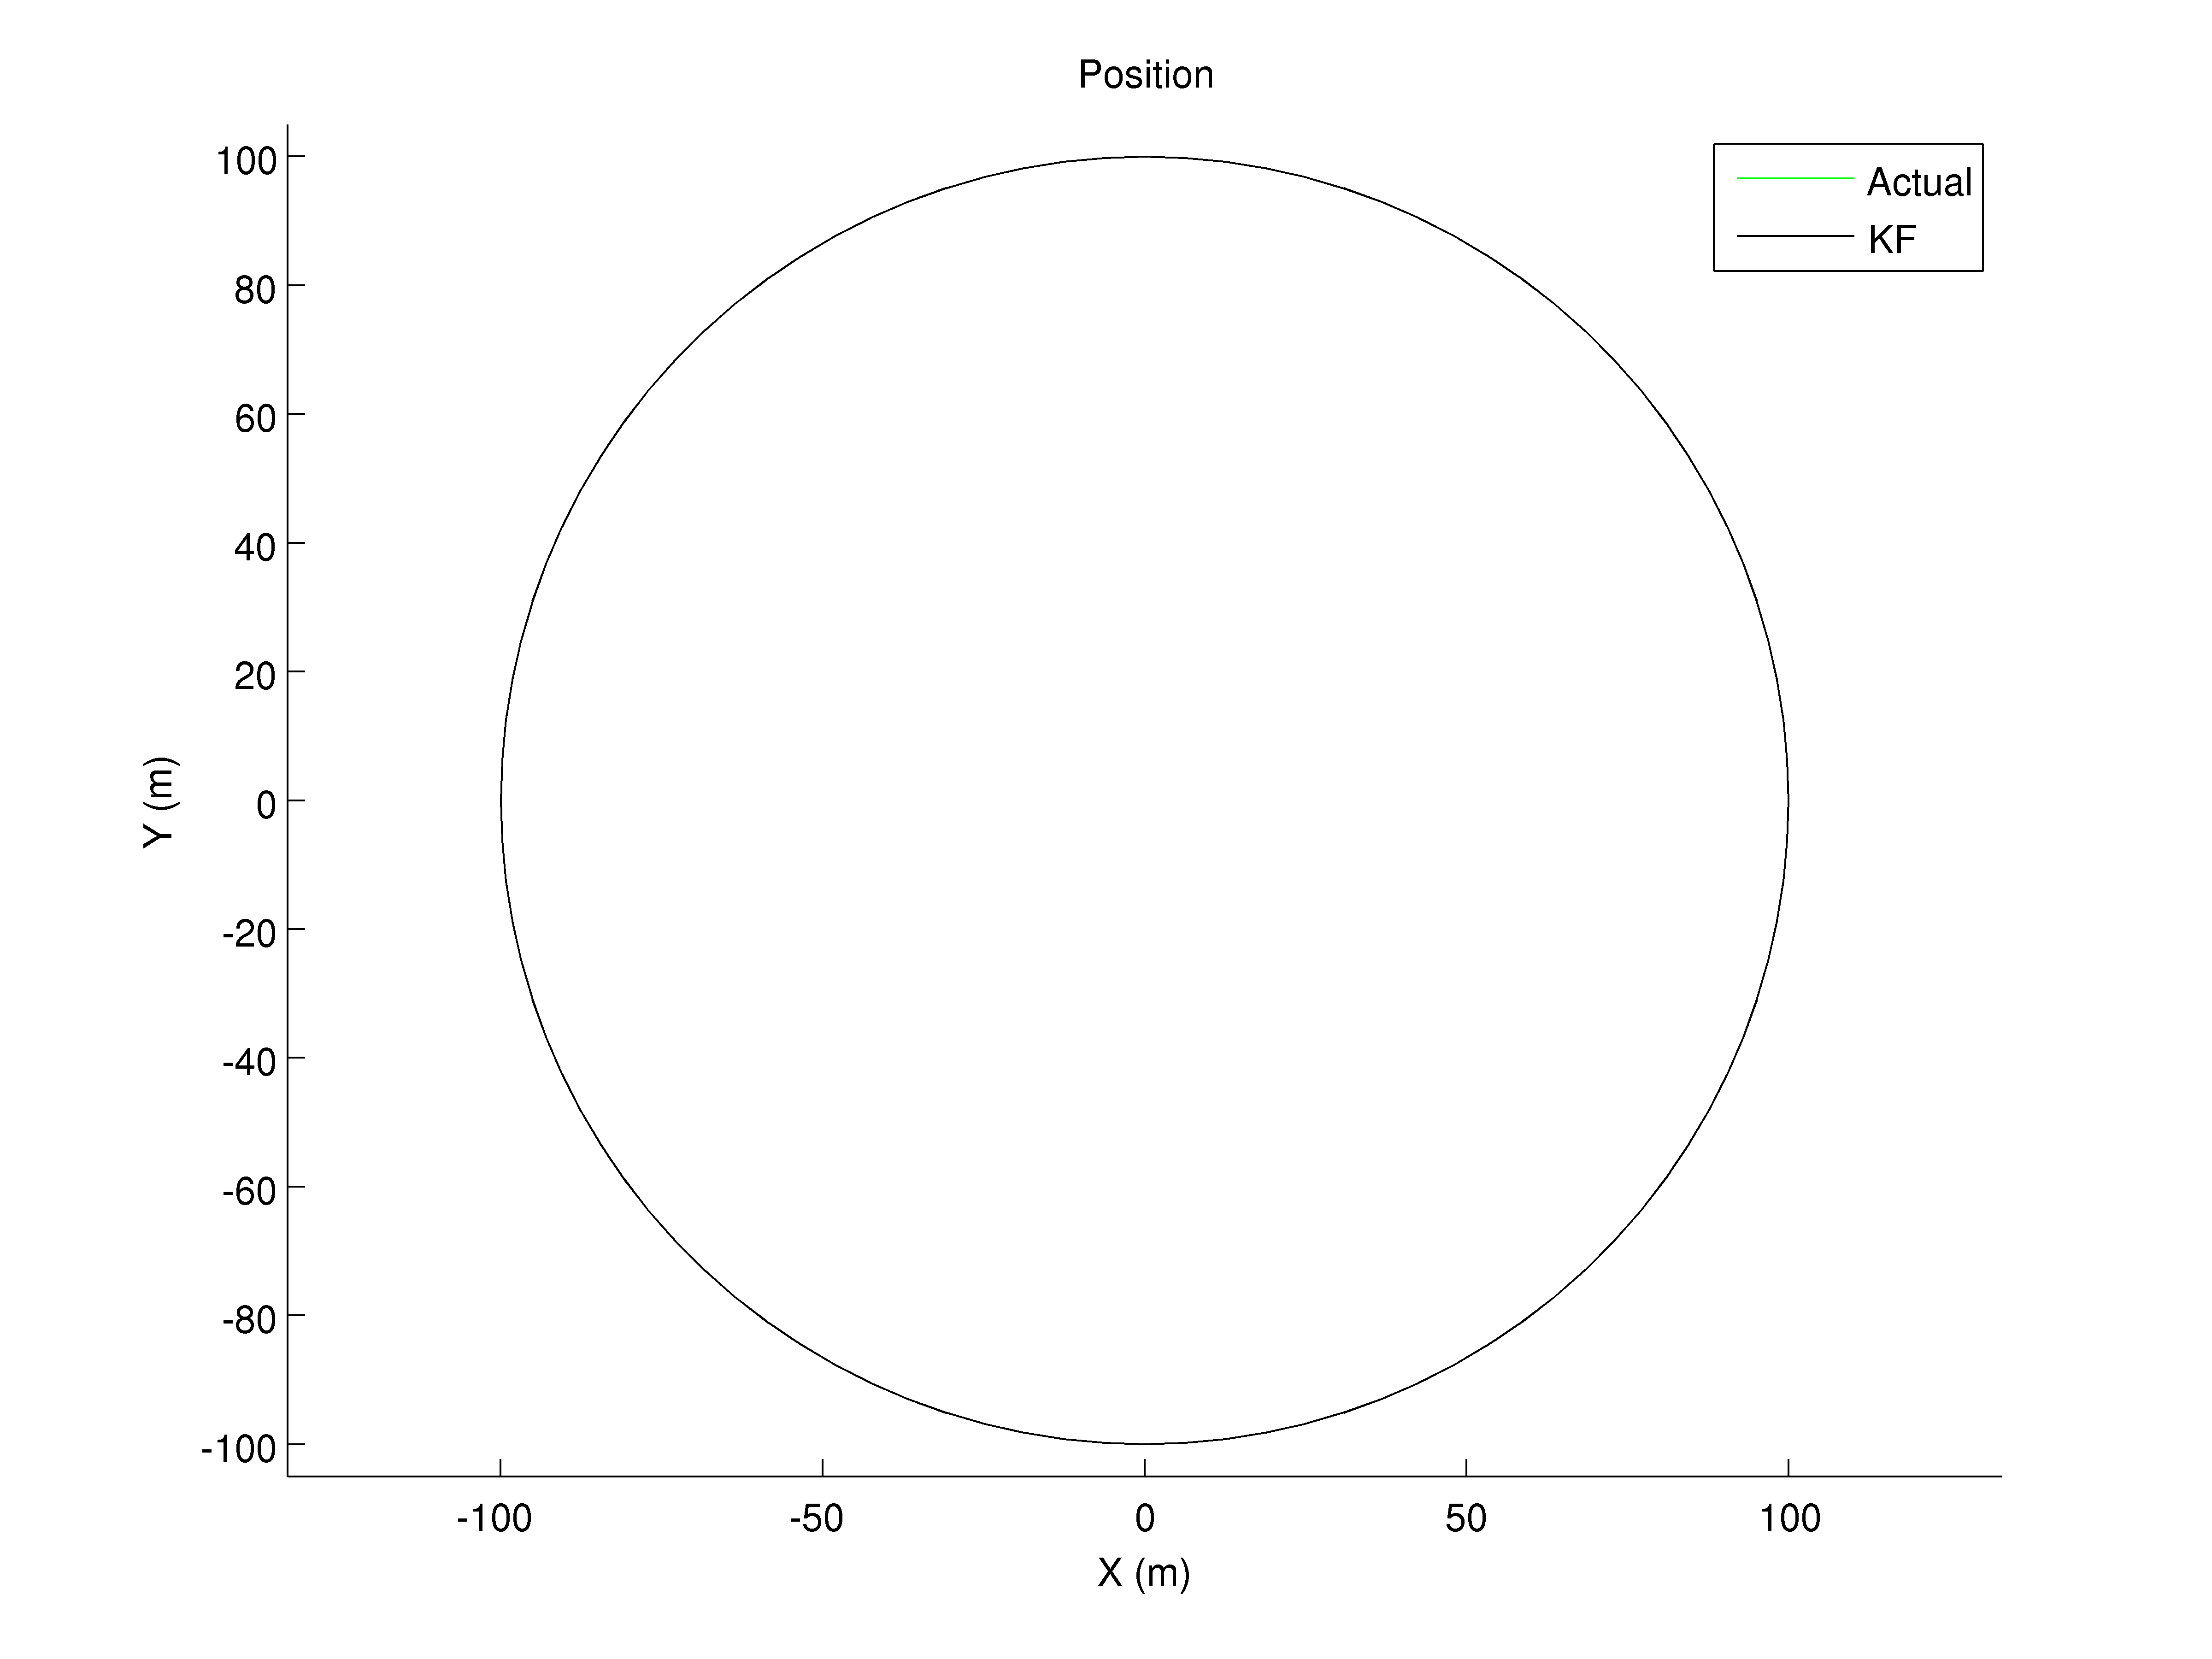
\includegraphics[width=.45\textwidth]{images/kfSimPosition} \\
    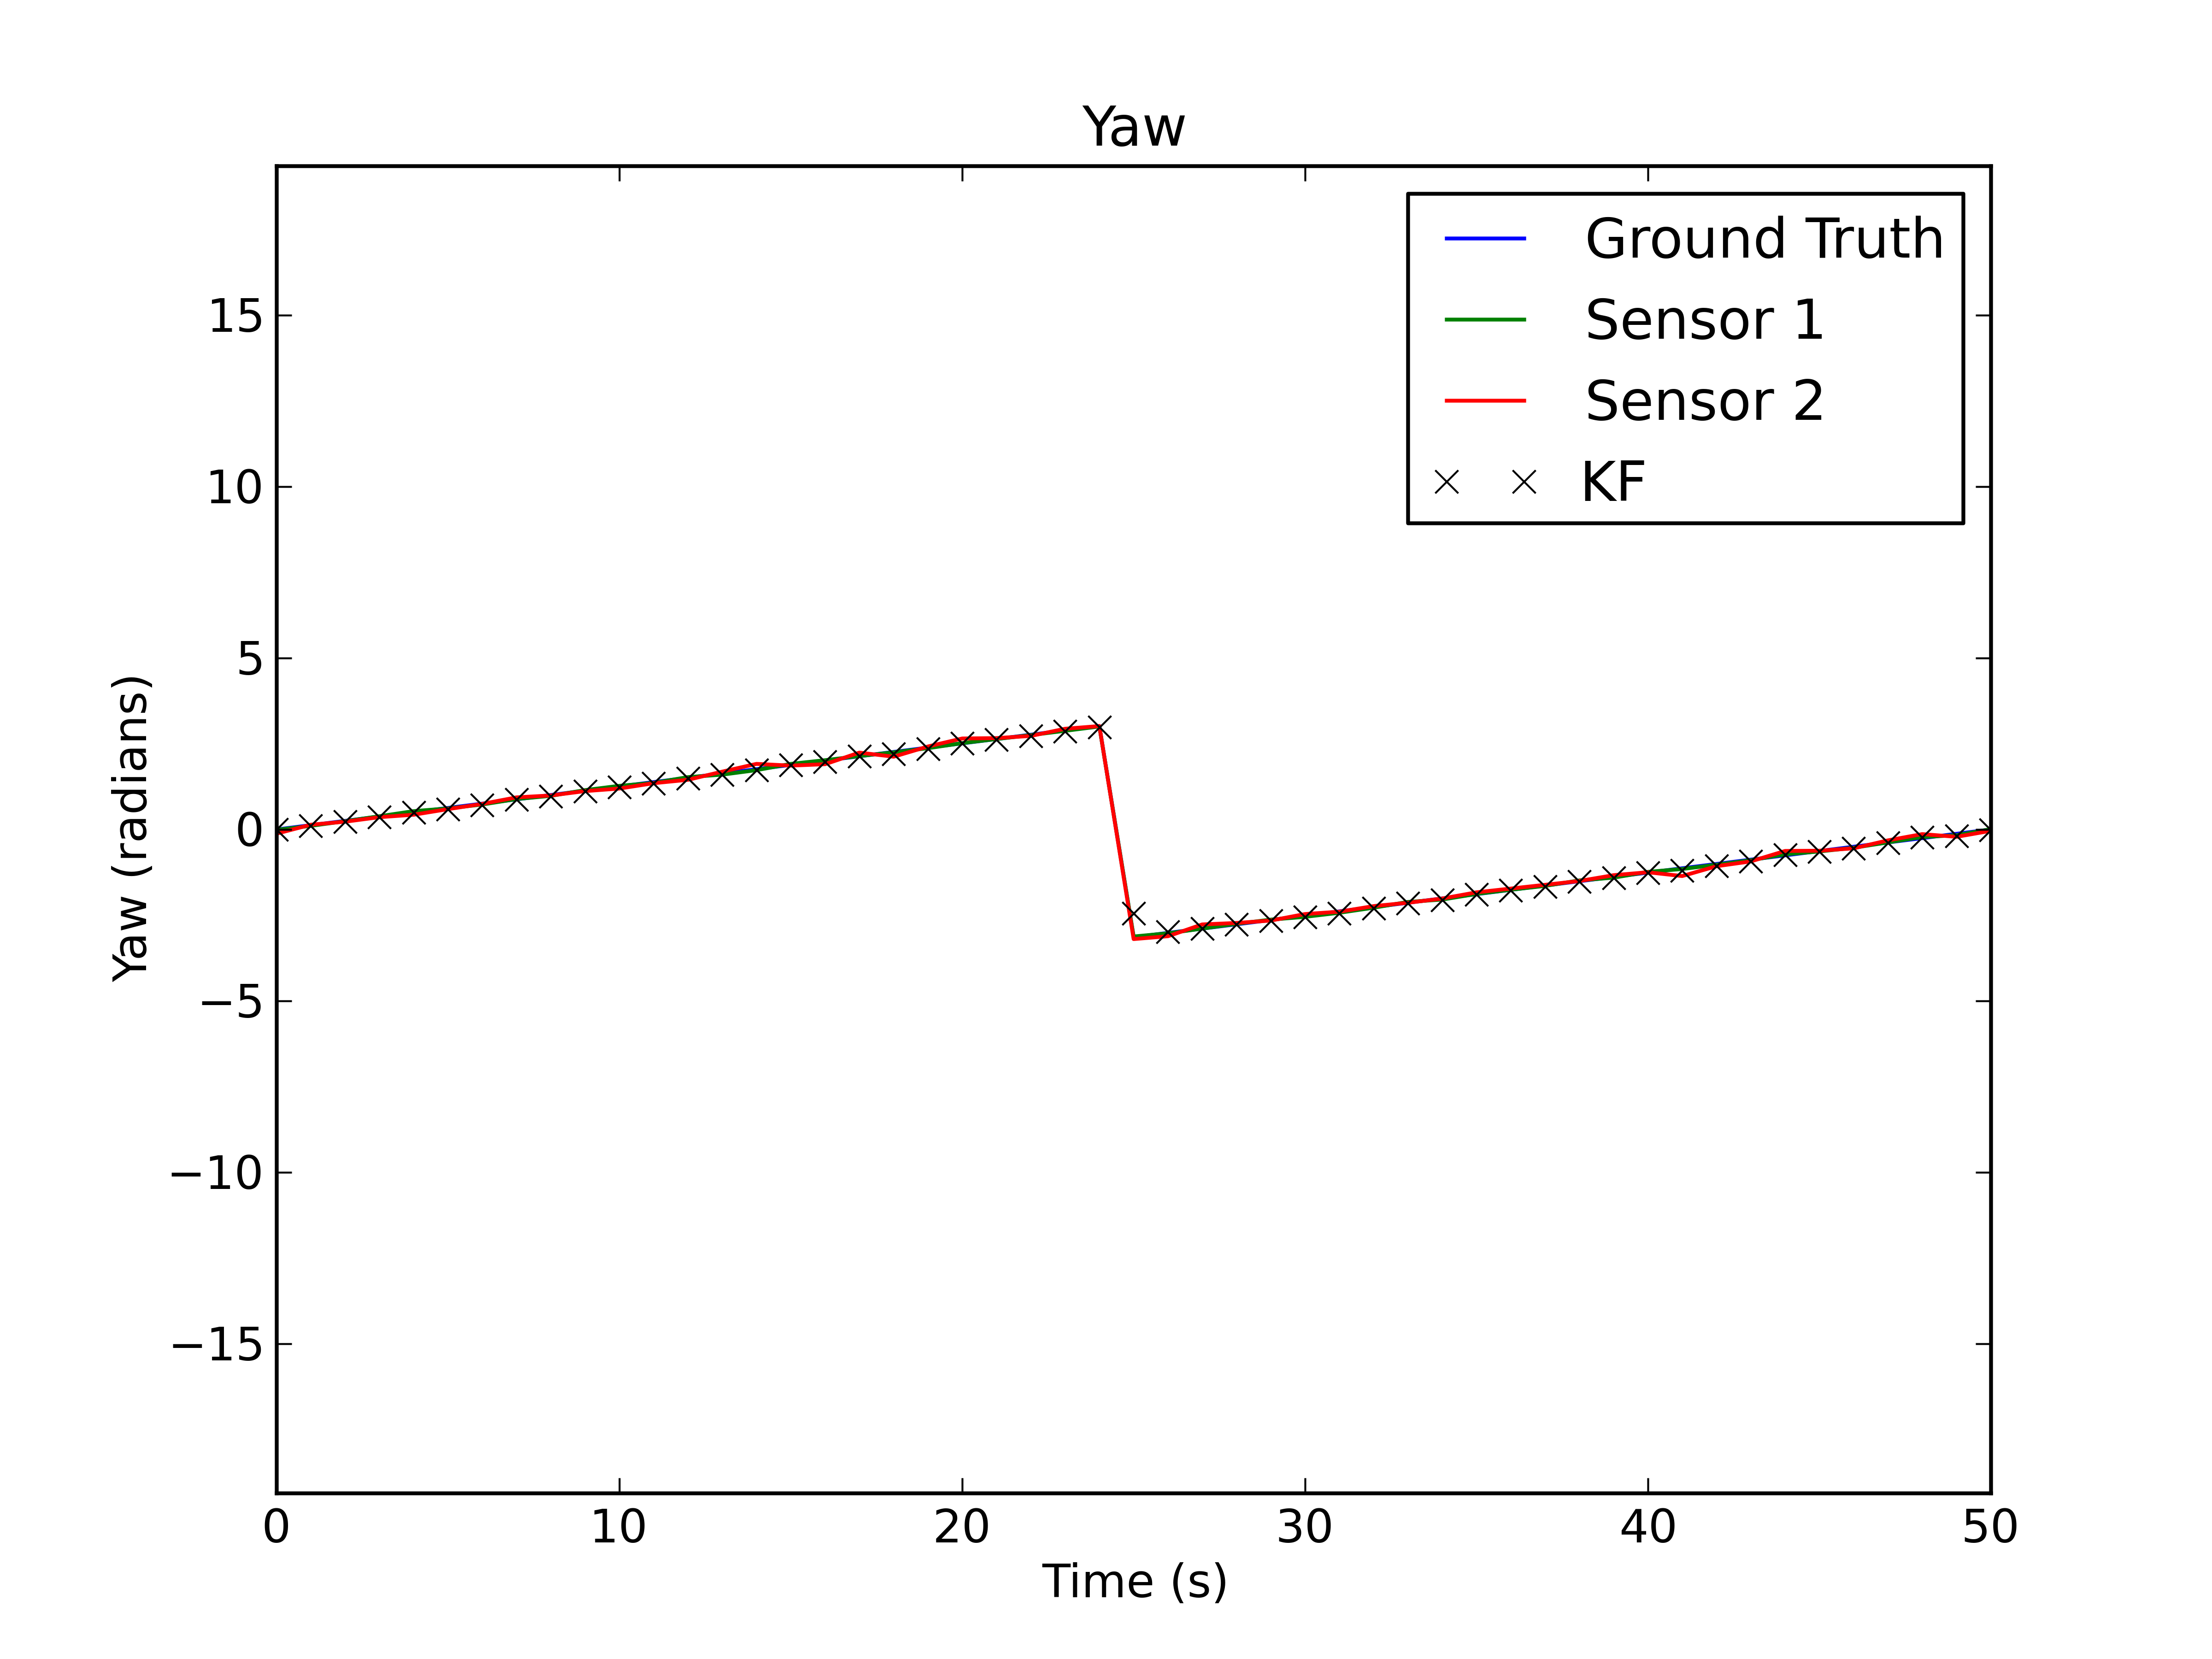
\includegraphics[width=.45\textwidth]{images/kfSimYaw} &
    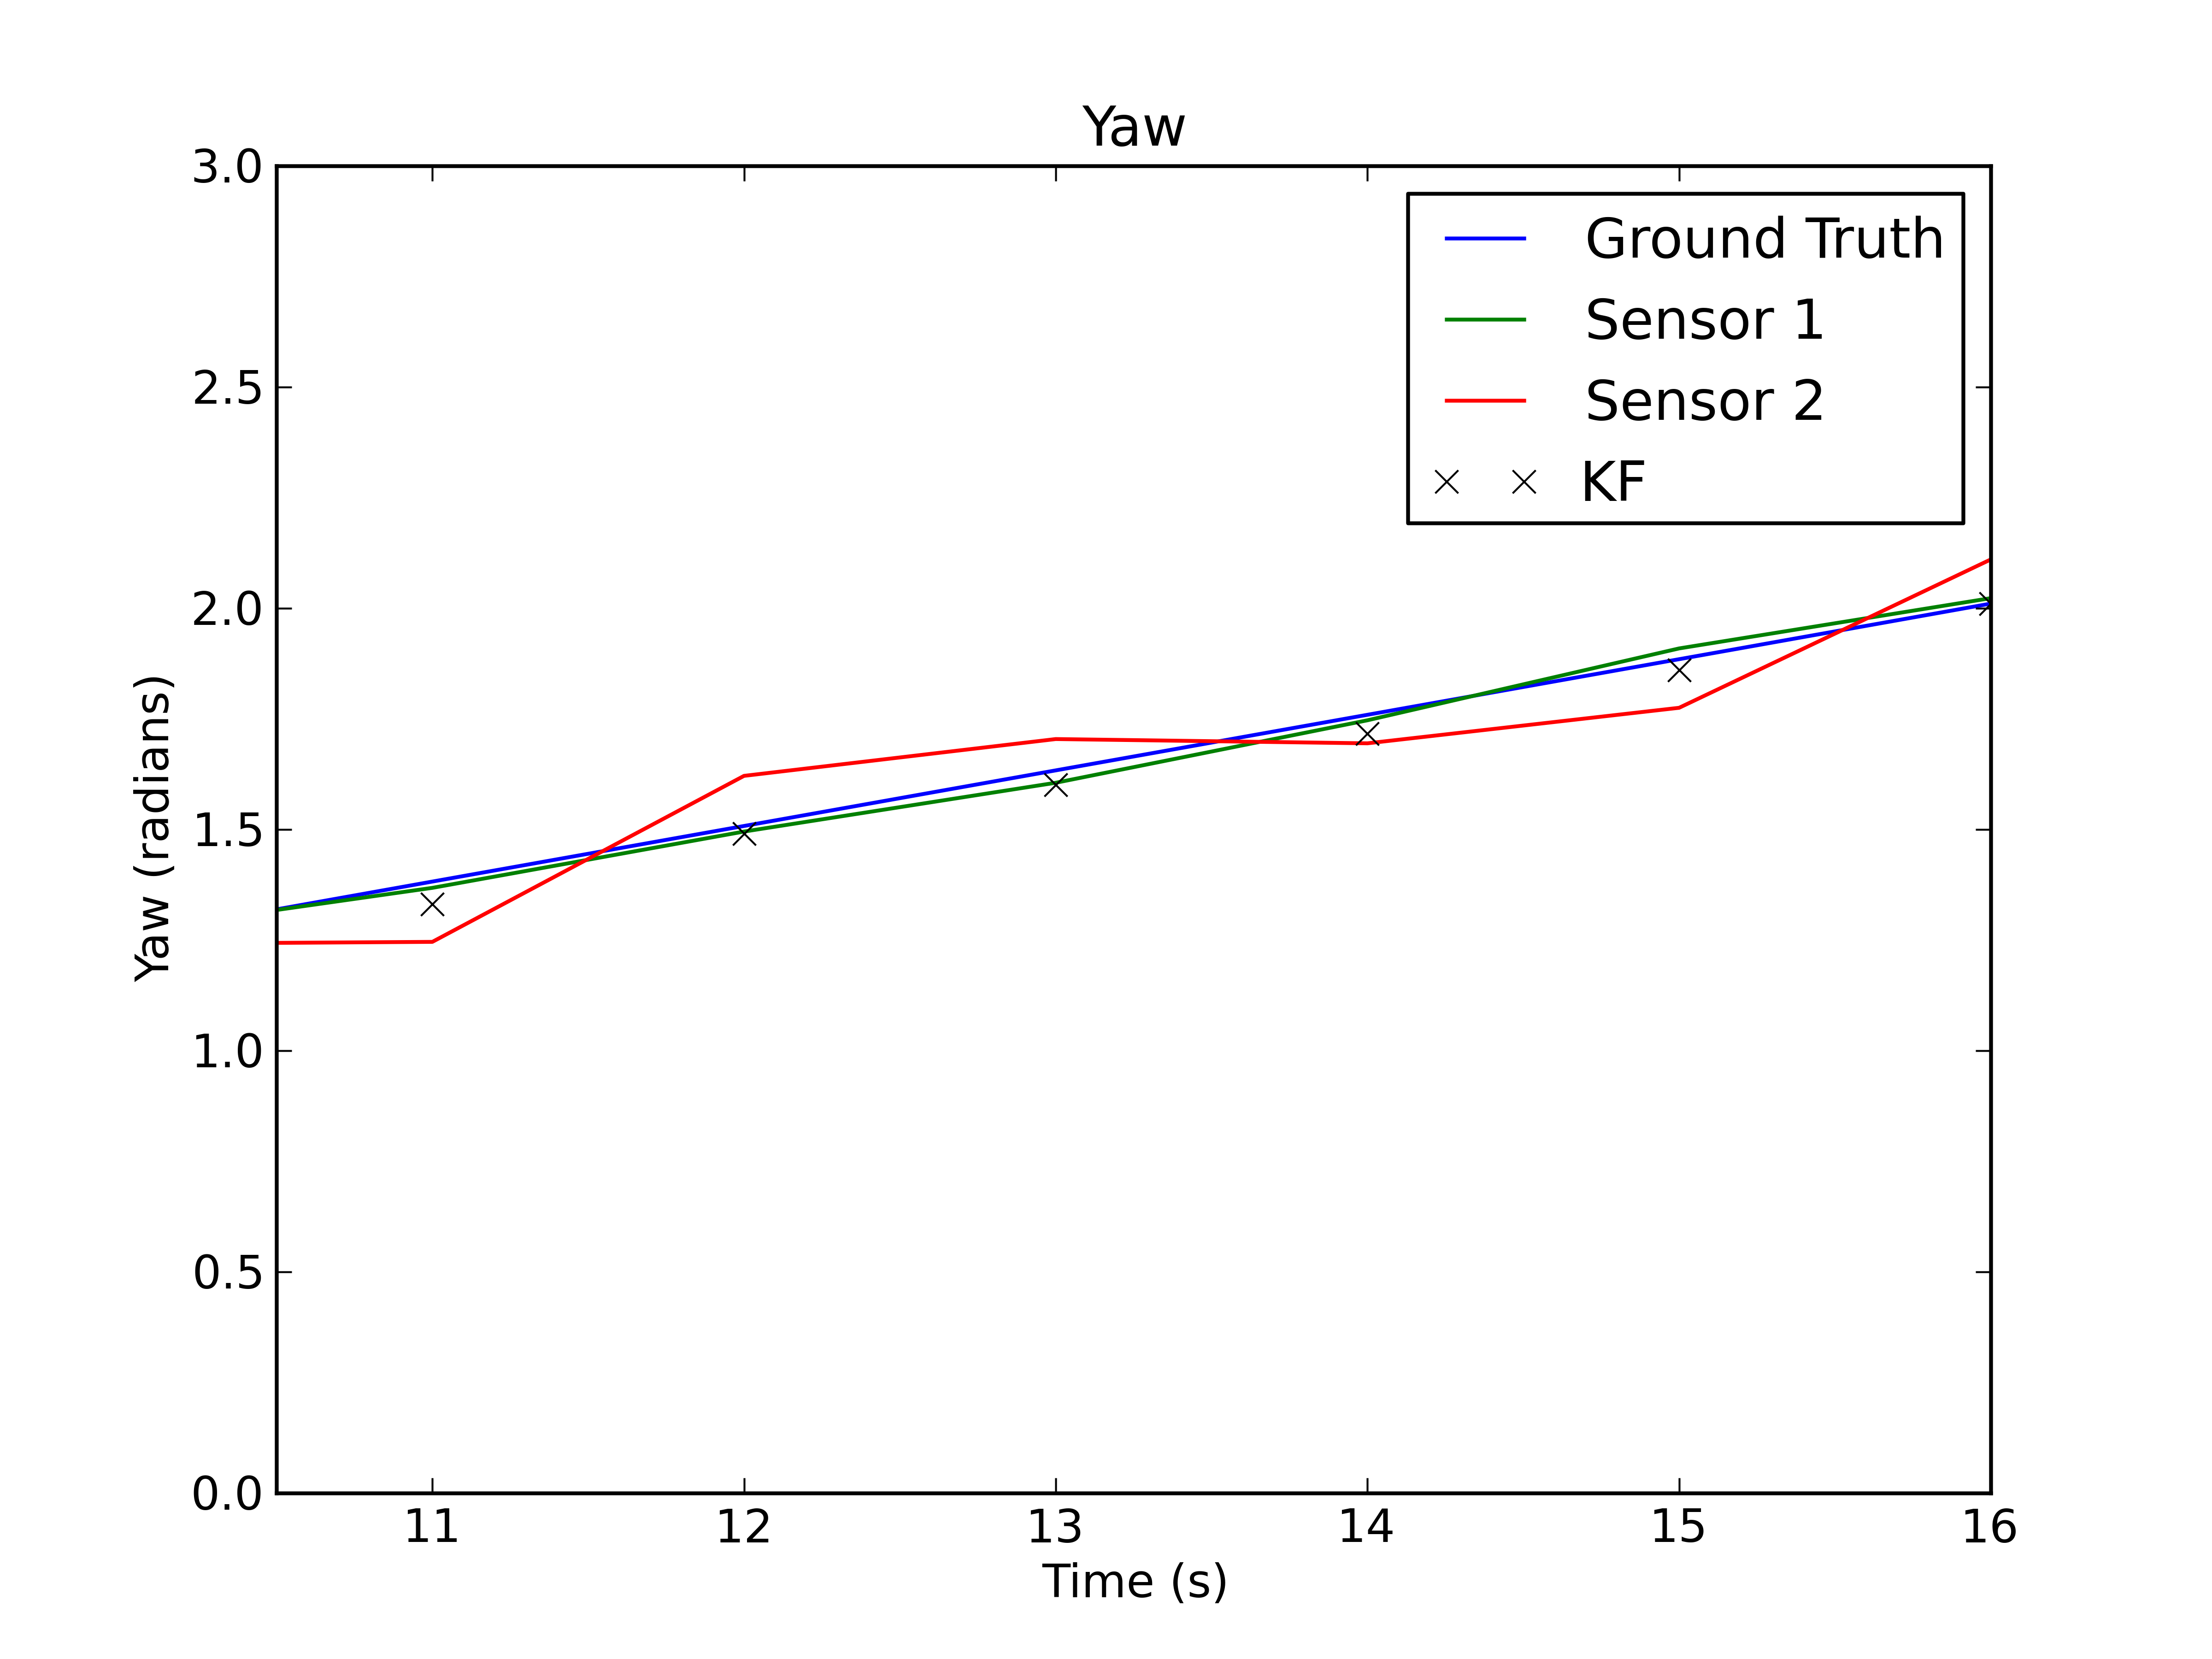
\includegraphics[width=.45\textwidth]{images/kfSimYawZoom}
    \end{tabular}
\end{figure}
\end{frame}

\begin{frame}{Evolution of Yaw Estimate Distribution}
\begin{center}
\begin{figure}[ht!]
\includemovie[poster, controls, repeat, text=(Loading movie...)]{6cm}{6cm}{code/kfdistribution.avi}
\end{figure}
\end{center}
\end{frame}

\begin{frame}{Effect of Noise Models on Estimate}
\begin{itemize}
\item KF performance is sensitive to parameter selection\footnote{Image from Busse \cite{Busse03adaptiveEKF}}.
\item Often very important to find correct covariance values.
\end{itemize}
\begin{figure}[ht!]
	\centering
	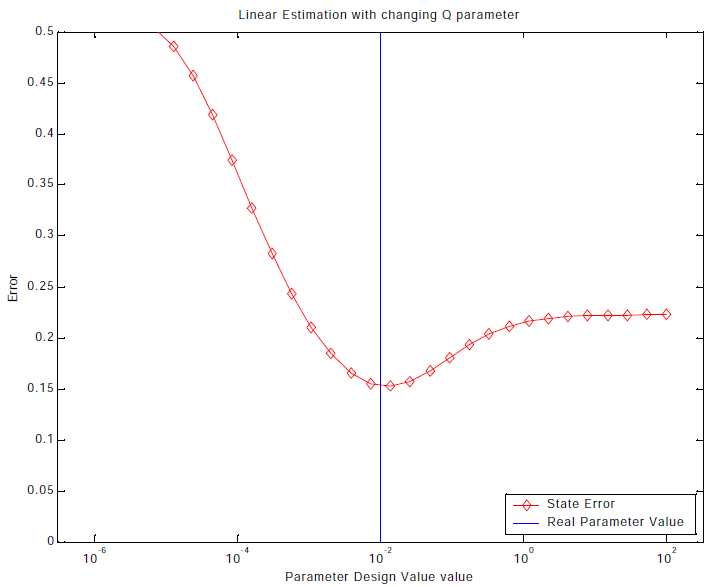
\includegraphics[width=.7\textwidth]{images/adaptiveSensitivity}
\end{figure}
\end{frame}

\begin{frame}{Adaptive EKF}
\begin{itemize}
\item Idea is to modify $Q$ and $R$ as data is collected.
\item Do \textit{not} want to adapt to static data, only run when velocity is non-zero.
\item Provides a running average based on difference between state and covariance estimates before and after measurement.
\end{itemize}
\begin{align*}
Q^\star &= \left(\hat{x}_k^+-\hat{x}_k^-\right)\left(\hat{x}_k^+-\hat{x}_k^-\right)^T + P_k^- - P_k^+ - \hat{Q}_k^- \\
\hat{Q}_k^+ &= \hat{Q}_k^- + \frac{1}{L_Q}\left(Q^\star-\hat{Q}_k^-\right) \\
R^\star &= \left(y_k-\hat{y}_k^+\right)\left(y_k-\hat{y}_k^+\right)^T - H_kP_k^+H_k^T \\
\hat{R}_k^+ &= \hat{R}_k^- + \frac{1}{L_R}\left(R^\star-\hat{R}_k^-\right)
\end{align*}
\end{frame}

\begin{frame}{Training KF Parameters}
\begin{itemize}
\item Idea is to log data, including ground truth, and replay through KF while adjusting $Q$ and $R$ to find best estimate compared to ground truth.
\item Use $Q$ and $R$ that generate the minimum error between estimate and ground truth.
\item One error metric minimizes only state errors, other minimizes combination of state errors and covariance.
\end{itemize}
\begin{align*}
\left<R_{\text{res}},Q_{\text{res}}\right> &= \argmin_{R,Q}\sum_{t=0}^T (y_t-h(\mu_t))^TP^{-1}(y_t-h(\mu_t)) \\
\left<R_{\text{pred}},Q_{\text{pred}}\right> &= \argmax_{R,Q}\sum_{t=0}^T -\log|2\pi\Omega_t| \\
&\qquad - (y_t-h(\mu_t))^T\Omega_t^{-1}(y_t-h(\mu_t)) \\
\Omega &= H_t\Sigma_tH_t^T+P
\end{align*}
\end{frame}

\begin{frame}{Alternate Estimation Methods}
\begin{itemize}
\item Augmented state Kalman filter to track sensor biases, state errors.
\item Kalman smoother in addition to Kalman predictor (prediction update step) and Kalman filter (measurement update step). Looks backward in time.
\item Unscented Kalman filter.
\item Central difference Kalman filter.
\item Sigma-point particle filter.
\item Adaptive Monte Carlo localization.
\item $H_\infty$ filter.
\end{itemize}
\end{frame}

\begin{frame}{Algorithm One Last Time}
\begin{itemize}
\item A generic system is represented by the model
\begin{align*}
x_{k+1} &= \Phi_kx_k + w_k \\
y_k &= H_kx_k + v_k
\end{align*}
\item Prediction update equations.
\begin{align*}
\hat{x}_{k+1}^- &= \Phi_k\hat{x}_k^+ \\
P_{k+1}^- &= \Phi_kP_k^+\Phi_k^T + Q_k
\end{align*}
\item Measurement update equations.
\begin{align*}
K_k &= P_k^-H_k^T\left[H_kP_k^-H_k^T + R_k\right]^{-1} \\
\hat{x}_k^+ &= \hat{x}_k^- + K_k\left[y_k - H_k\hat{x}_k^-\right] \\
P_k^+ &= \left[I - K_kH_k\right]P_k^-
\end{align*}
\end{itemize}
\end{frame}

\begin{frame}{Kalman Filter Derivation}
\begin{itemize}
\item Good derivation at \\
\href{http://www.aticourses.com/kalman\_filter.pdf}{http://www.aticourses.com/kalman\_filter.pdf}
\end{itemize}
\end{frame}

\begin{frame}[allowframebreaks]{References}
\nocite{Sights06}
\nocite{Kelly_1994_338}
\nocite{Orderud05}
\nocite{Simon06OptimalEstimation}
\nocite{Busse03adaptiveEKF}
\nocite{Mehra72}
\nocite{Merwe04sigma-pointNavigation}
\nocite{Busse03adaptiveEKF}
\nocite{Abbeel05discriminativetraining}
\nocite{Gelb74}
\nocite{AndersonMoore79}
\nocite{KalmanOriginal60}
\nocite{KalmanBucy61}
\bibliographystyle{plain}
\bibliography{mybib}
\end{frame}

%\begin{frame}{General Kalman Filter Assumptions}
%\begin{itemize}
%\item Linear systems.
%\item Random variables have Gaussian distributions.
%\item Any noise in the system model or sensor data is white noise.
%\item All processes are Markov processes.
%\item Assumptions allow for specific, fairly easy to calculate equations for state and covariance propagation with low memory requirements.
%\end{itemize}
%\end{frame}

\begin{frame}{Linear Algebra Basics}
\begin{itemize}
\item Matrix-vector multiplication goes left-to-right, top-to-bottom:
\begin{align*}
\left[\begin{array}{c c}
a & b \\ c & d
\end{array}\right]
\left[\begin{array}{c}
e \\ f
\end{array}\right] &=
\left[\begin{array}{c}
a*e + b*f \\ c*e + d*f
\end{array}\right] \\
\Rightarrow \left[\begin{array}{c c}
2 & 4 \\ 1 & 7
\end{array}\right]
\left[\begin{array}{c}
3 \\ 9
\end{array}\right] &=
\left[\begin{array}{c}
2*3 + 4*9 \\ 1*3 + 7*9
\end{array}\right] =
\left[\begin{array}{c}
42 \\ 66
\end{array}\right]
\end{align*}
\item Matrix-matrix multiplication goes left-to-right, top-to-bottom:
\begin{align*}
\left[\begin{array}{c c}
a & b \\ c & d
\end{array}\right]
\left[\begin{array}{c c}
e & f \\ g & h
\end{array}\right] &=
\left[\begin{array}{c c}
a*e + b*g & a*f + b*h \\ c*e + d*g & c*f + d*h
\end{array}\right] \\
\Rightarrow \left[\begin{array}{c c}
2 & 4 \\ 1 & 7
\end{array}\right]
\left[\begin{array}{c c}
3 & 2 \\ 9 & 1
\end{array}\right] &=
\left[\begin{array}{c c}
2*3 + 4*9 & 2*2 + 4*1 \\ 1*3 + 7*9 & 1*2 + 7*1
\end{array}\right] \\
&= \left[\begin{array}{c c}
42 & 8 \\ 66 & 9
\end{array}\right]
\end{align*}
\item Matrices are upper-case, vectors are lower-case.
\end{itemize}
\end{frame}

%\begin{frame}{Linear Models}
%\begin{itemize}
%\item A linear model supports superposition and scaling.
%\item Superposition means variables can be added together.
%\item Scaling means a common multiplier can be moved outside the addition.
%\item Example:
%\end{itemize}
%\begin{align*}
%y_1(t) &= H\{x_1(t)\} \\
%y_2(t) &= H\{x_2(t)\} \\
%\Rightarrow \alpha y_1(t) + \beta y_2(t) &= \alpha H\{x_1(t)\} + \beta H\{x_2(t)\} \\
%&= H\{\alpha x_1(t) + \beta x_2(t)\}
%\end{align*}
%\end{frame}

%\begin{frame}{Random Variables}
%\begin{itemize}
%\item Random variables have a distribution that describes the probability that the variable will have a particular value at a given time.
%\item If variables are truly random and can take \textit{any} value then no prediction method will work.
%\item Kalman filters assume that variables have Gaussian distributions.
%\item Gaussian random variables can be described entirely by a mean and a variance (the first two moments) and are represented using the notation $x\sim\mathcal{N}(\mu,\sigma^2)$ where $\mu$ is the mean and $\sigma^2$ is the variance. $\sigma$ is the standard deviation.
%\end{itemize}
%\end{frame}

%\begin{frame}{Gaussian Distribution}
%\begin{itemize}
%\item The probability distribution funtion for Gaussian random variables\footnote{Image from Wikipedia.}.
%\item Can be recreated knowing only the mean and variance.
%\end{itemize}
%\begin{figure}[ht!]
%    \centering
%    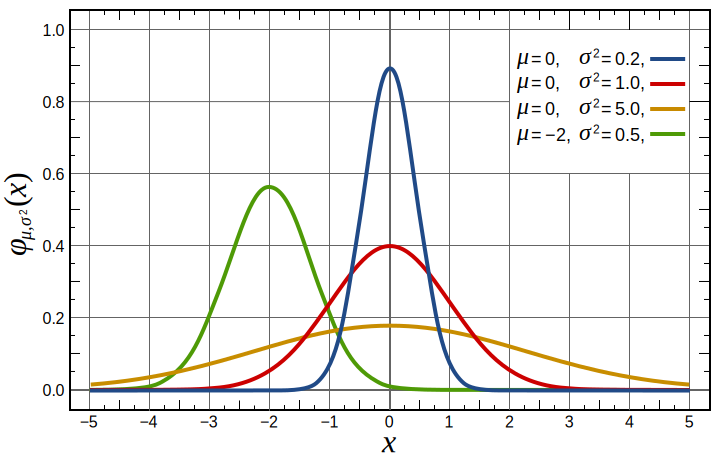
\includegraphics[width=.5\textwidth]{images/Normal_Distribution_PDF}
%\end{figure}
%\end{frame}

%\begin{frame}{Noise}
%\begin{itemize}
%\item Noise can be described by a distribution.
%\item Kalman filters assume that all noise is white noise with zero mean.
%\item White noise is statistically uncorrelated with itself\footnote{Image from Wikipedia.}.
%\item White noise \textit{does not exist}.
%\item Colored noise can be filtered to make it seem white.
%\item Most noise is "close enough" to white that the assumption is typically valid.
%\end{itemize}
%\begin{figure}[ht!]
%    \centering
%    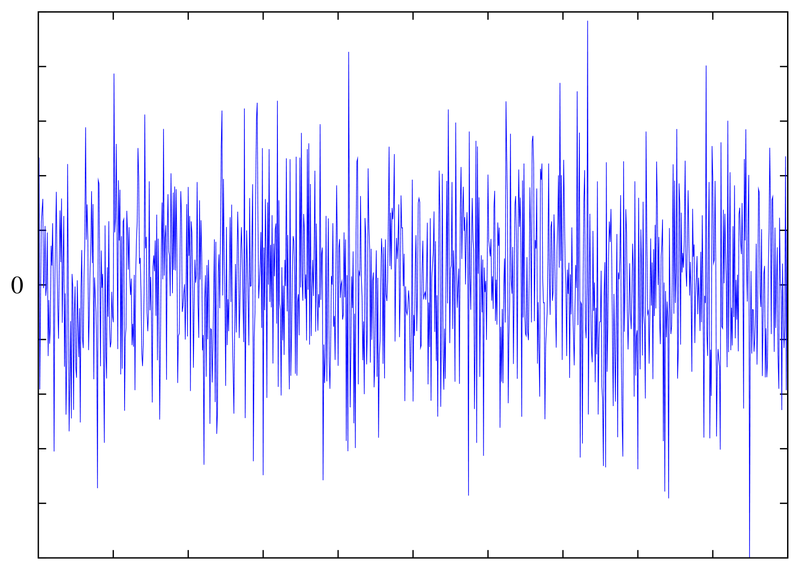
\includegraphics[width=.4\textwidth]{images/WhiteNoise}
%\end{figure}
%\end{frame}

%\begin{frame}{Markov Processes}
%\begin{itemize}
%\item A Markov process is one which is known only by its current state.
%\item No history needs to be recorded.
%\item Example is a moving car. If you know a cars position, orientation, velocity and acceleration then you don't need to know if it stopped at the grocery store to know where the car will be in 10 seconds.
%\item Valid for a very large number of processes including estimating the state of robots.
%\end{itemize}
%\end{frame}

%\begin{frame}{How Good Is The Estimate?}
%\begin{itemize}
%\item The covariance of the state estimate $\hat{x}_k$ is computed to give an idea of how good the state estimate is.
%\begin{align*}
%P_{k+1}^- &= \Phi_kP_k^+\Phi_k^T + Q_k
%\end{align*}
%\item $P$ gives a confidence value for the calculated states that weights how much trust should be put into the model-based estimate when new sensor data is received.
%\item $Q$ is a matrix with the covariance values of the states in the system model.
%\end{itemize}
%\end{frame}

%\begin{frame}{States and Covariances}
%\begin{itemize}
%\item The Kalman filter is built on the idea that states and covariances can be calculated through time.
%\item Since the Kalman filter assumes Gaussian distributions and Markov processes only the state and variance need to be tracked.
%\end{itemize}
%\end{frame}

%\begin{frame}{State Propagation}
%\begin{itemize}
%\item Talk about how state estimates are calculated through time.
%\end{itemize}
%\end{frame}

%\begin{frame}{Covariance Propagation}
%\begin{itemize}
%\item Talk about how covariances are calculated through time.
%\end{itemize}
%\end{frame}

\end{document}
